\documentclass[UTF8]{swputhesis}
\usepackage{hyperref}
\usepackage{biblatex}
\usepackage[nameinlink]{cleveref}  % after hyperref package
\usepackage{subfig}  % for subfigures

% 代码格式设置
\usepackage{listings}
\usepackage[dvipsnames]{xcolor}


% 在导言区进行样式设置
\lstset{
    language=Python, % 设置语言
	basicstyle=\ttfamily, % 设置字体族
	breaklines=true, % 自动换行
	keywordstyle=\bfseries\color{NavyBlue}, % 设置关键字为粗体,颜色为 NavyBlue
	morekeywords={}, % 设置更多的关键字,用逗号分隔
	emph={self}, % 指定强调词,如果有多个,用逗号隔开
    emphstyle=\bfseries\color{Rhodamine}, % 强调词样式设置
    commentstyle=\itshape\color{black!50!white}, % 设置注释样式,斜体,浅灰色
    stringstyle=\bfseries\color{PineGreen!90!black}, % 设置字符串样式
    columns=flexible,
    numbers=left, % 显示行号在左边
    numbersep=2em, % 设置行号的具体位置
    numberstyle=\footnotesize, % 缩小行号
    frame=single, % 边框
    framesep=1em % 设置代码与边框的距离
}
 


\graphicspath{{fig/}} % 设置插图文件存放位置
\addbibresource{ref.bib} % 设置参考文献文件位置

% 图书分类号:在 https://www.clcindex.com/ 查询
\clc{TE319}
\ctitle{基于提示工程的文本主题建模框架}
\cmajor{专业学位硕士}
\cdomain{计算机技术}
\research{研究方向}
\cauthor{蒋鹏}
\id{202125000062}
\csupervisor{肖斌}
\cwsupervisor{}

% 英文封面,暂不要求
% \etitle{TITLE TITLE TITLE TITLE TITLE TITLE}
% \emajor{major}
% \eauthor{author name}
% \esupervisor{supervisor name}
% \edate{June, 2021}

\degree{专业学位} % 学位类型,可选:学术学位、专业学位。该设置会影响封面及页眉
\cdate{2025年6月}

\begin{document}

% 封面(由于学术硕士和专业硕士论文封面不同,建议使用 word 制作封面)
\makecover

% 版权声明与独创性声明
\makecopyright

% 摘要、目录页
\frontmatter

% 摘要
\begin{cabstract}
    图像分割是一个计算机视觉领域实现对图像分析的基础领域,但伴随数据量的剧增、图像场景越来越复杂,单一的图像语义或实例分割无法满足多数计算机视觉的任务需求,因此全景分割应运而生。全景分割利用语义标签和实例特征实现对图像场景的全面理解。当前高精度全景分割方法计算量大,导致高效方法不能满足实际应用的时效需求。精度和耗时的冲突已成为二维图像和三维激光雷达图像全景分割技术,在部署自动驾驶应用场景中瓶颈。为缓解此问题,本文开展了如下研究:首先采用一种基于像素级实例感知的全景分割方法,用于提高基于单阶段架构的二维图像全景方法的分割精度。该方法利用FPN(Feature Pyramid Network,特征金字塔网络)对输入图像进行多尺度特征信息提取,再将多尺度特征图分别传入语义分支、目标检测分支和全景分支。网络中使用FCOS(Fully Convolutional One-stage,全卷积单阶段)目标检测器为全景分支提供实例中心信息,辅助像素级实例感知掩码生成,语义分支为全景分支提供标签。基于所属方法获得高精度分割效果的同时,使用语义分支与全景分支乘积作为全景分割结果,减少了后处理融合耗时。本研究选择Cityscapes数据集(包含超过5000张像素图像)用以实验。 
    该方法不仅完成了基于特征金字塔和像素级实例感知掩码提高全景分割精度的任务,还实现了使用语义分支与全景分支乘积融合代替传统融合处理减少计算耗时的目的,缓解了全景分割方法精度和效率之间的经典折衷问题。在Cityscapes数据集上实验论证了所属方法的良好分割效果,为自动驾驶等计算机视觉任务的进一步应用,丰富了可用于图像分割技术手段。

    摘要题头应居中,小二号黑体 (与章标题格式相同)。
    摘要要求为写实性的叙述,阐明研究意义、理论方法、开展的工作、取得成果和认识,最好给出定量性的结论。
    英文摘要应与中文内容一致,表述得体。

    摘要文字后空一行,顶格 (即不缩进) 写出关键词。``关键词:'' 用小四号、黑体,
    而关键词内容用小四号、宋体,内容 3 $\sim$ 5 个,关键词之间用  ``;'' 隔开。

    ``Key words'' 没给出格式规定,几个 Word 模板都有不同,有采用宋体,有采用黑体的,
    这里暂时采用了宋体加粗。

    \ckeywords{西南石油大学;硕士论文;模板;深度学习;全景分割;卷积神经网络;特征金字塔网络;FCOS目标检测器}

\end{cabstract}

\begin{eabstract}
    The abstract is an important component of your thesis. Presented at the
    beginning of the thesis, it is likely the first substantive description of
    your work read by an external examiner. You should view it as an opportunity
    to set accurate expectations.

    The abstract is a summary of the whole thesis. It presents all the major
    elements of your work in a highly condensed form.
    An abstract often functions, together with the thesis title,
    as a stand-alone text.

 
    \ekeywords{Deep learning; Panoramic segmentation; Feature Pyramid Network; Convolutional neural network; FCOS target detector}
\end{eabstract}


% 生成目录
\tableofcontents

% 正文
\mainmatter

% 这一章节主要是介绍和测试论文格式,也可以用于快速学习 LaTeX 写作的基本用法
% 阅读完这一格式章节后删除这一行, 以及删除 src/format.tex 文件
\include{src/format}

% 正文部分,可自行添加章节
% !TEX root = ../swputhesis.tex
\chapter{绪论}
\section{研究背景与意义}
长期以来,交通事故常常是由于人类驾驶员的错误操作而导致的,这给人们带来了人员伤亡和经济损失。为了解决这个问题,研究人员引入了自动驾驶的概念,旨在提高汽车乘员的安全性和舒适性\cite{秦飞巍2021无人驾驶中的场景实时语义分割方法}。自动驾驶是指在智能系统的控制下驾驶汽车,实现准确决策的智能系统需要具备场景理解的能力。全景分割技术可以作为一种出色的方法,因为从摄像头获取的图像需要经过处理才能理解场景\cite{everingham2010pascal}。

在这个领域,已经存在各种全景分割方法,其中一些试图在准确性和速度之间取得平衡。然而,正确识别对象边界内的像素标签和考虑不同比例的对象是两个具有挑战性的问题,使得这些架构难以达到高准确性。

语义分割是计算机视觉领域中的一项重要任务,其目标是将输入的图像分割成多个语义区域,并为每个像素分配一个语义标签,以确定其所属的语义类别。与传统的图像分割任务不同,语义分割需要对每个像素进行分类,而不仅仅是将图像分割成不同的区域。例如,在街景图像中,语义分割可以将图像分成道路、建筑、车辆、行人等多个语义区域,并为每个像素指定其所属的语义类别。语义分割在自动驾驶、物体识别、场景理解等领域具有广泛的应用。

实例分割是一种将目标检测和语义分割结合起来的技术,它仅针对图像中的目标进行检测,并对检测到的目标进行精细分割。与目标检测中的边界框相比,实例分割能够提供更精确的物体边缘信息\cite{kirillov2019panoptic}。
日常生活中发生着很多基于全景分割技术完成图像生成的应用,尤其是近年来蓬勃发展的自动驾驶车辆有关研究,在车辆行进过程中,自动驾驶技术首先获取到车辆、行人和其他移动物体信息,基于这些信息构建调控模型,再依据这些信息完成对车辆转向、刹车、速度的自动控制。目前汽车信息感知常用毫米波雷达和激光雷达,这些感知器将微波或激光发射到大气中后,接收障碍物反射的信号后进行处理,虽然这类技术具有较高的障碍物识别性能,但缺乏进一步提供车辆周围障碍物的分析能力,例如周围障碍物的大小和运动信息。为解决该问题,模仿人类使用触觉和视觉识别周围环境的模式,越来越多的自动驾驶技术在保留雷达感知技术的基础上,引入了前置摄像头增强车辆感知技术,通过对相机所得图像执行分割来增强驾驶环境信息。近年来,深度学习在计算机视觉领域的巨大发展,大大提升了机器实现图像识别的精度和性能,也很众多分类和全景分割网络神经网络\cite{wangye}被用于增强车辆自动驾驶的可靠性。图像的准确分割和理解建模已逐渐成为自动驾驶技术承上启下的关键调控技术,许多学者深耕于结合低耗时实现图像的高精度分割。

全景分割是将语义分割和实例分割相结合的技术,旨在对图像中的所有物体和背景进行检测和分割\cite{he2017mask}。与仅对感兴趣的目标区域进行分割的实例分割不同,全景分割需要对整个图像进行完整的分割,包括背景区域的分割。在全景分割中,背景区域的分割属于语义分割,而物体的分割则属于实例分割\cite{wu2019wider}。

图像分割主要有三种方式,即实例分割、语义分割和全景分割,它们之间存在一定的关联:
(1)实例分割:将图像中的每个对象分割出来,并将其转换为不同的实例。例如,在一张图像中有人和动物,可以将人和动物的轮廓分割成不同的实例\cite{he2017mask}。
(2)语义分割:将具有相同语义类型的图像区域分割成不同的区域,确保区域之间没有重叠。例如,对于街景图像,可以将道路、天空、建筑物等元素利用语义分割成多个区域\cite{long2015fully}。
(3)全景分割:对图像中每个像素的标签进行预测,并按照类别对像素进行分类,使得每个像素都有对应的语义类别。全景分割是语义分割和实例分割的综合称呼,在全景分割过程中,每个对象和像素都必须经过实例和语义分割才能预测标签。

总的来说,全景分割包括了实例分割和语义分割,如果能够同时预测每个像素的标签和实例编号,就能得到完整的全景分割图像。

当前主流的全景图像分割体系结构主要包括自上而下、自下而上和单径结构。自上而下的体系结构可以进一步划分为单相和双相模型\cite{he2017mask}。在自上而下的全景图像分割方法基础上,引入了一种新的图像分割方法。该方法采用两级图像分割模式,首先利用二级神经网络对一级图像进行后处理,然后再对一级图像进行后处理,实现全景图像的分割。为了减少自顶向下两阶段全景分割模型的计算复杂度,自顶向下单阶段全景分割模型省略了建议生成阶段,仅基于单阶段的目标检测来进行分割。此外,还采用了自下而上的方式,对原始影像中的每个像素进行义项分类,然后通过群组聚类的方式,在相同的义项下实现对不同样本的判别。无论是自上而下还是自下而上的全景图像分割算法,都是基于两条路径,即语义和实例路径,将物体与背景分离。而完整卷积单路径则将实例与背景的分割统一起来。

\section{全景分割图像生成}
在现实生活中,基于全景分割的图像生成应用非常广泛。例如,在自动驾驶领域,通过感知车辆、行人和移动物体等障碍物,来控制车辆的加速度。自动驾驶系统通过识别驾驶环境中的要素,如道路、车道、交通信号灯和标志,来确定车辆的行驶方向。为了实现准确的障碍物识别,汽车中使用的雷达和激光雷达可以发送微波或激光,并接收和处理障碍物反射的信号。然而,它们无法提供复杂的环境信息,如道路边界和车道分类。为了获取更详细的驾驶环境信息,前置摄像头成为必要的传感器之一,它通过处理图像来提供驾驶环境信息,就像人们通过视觉来认知周围环境一样。近年来,深度学习的发展极大地提升了图像识别性能,因此被应用于对车辆的高可靠性需求中的分类和全景分割网络。

对图像的准确理解和建模一直以来都备受关注,因为精确的场景模型是实现智能安防和自动驾驶等高层任务的基础。目前,像素级的场景理解主要包括实例分割和语义分割,而全景分割作为一种新提出的技术,统一了这两个任务,推动了对场景的全面理解。

随着深度学习的引入,处理大量可视化数据已变得相当可行、准确和高效。深度学习在图像分类等许多领域中优于传统技术,如目标检测、目标识别和语义分割。对自然场景的理解在很大程度上依赖于实例分割,其目标是对图像中的每个像素进行分类,并为其分配一个类别标签。实例分割可以被看作是一个针对图像中每个像素进行密集分类的问题,而不是一次对整个图像进行处理。尽管深度学习在许多应用中表现优秀,但成功需要大量的训练数据,比传统方法所需的数据量要高出一个数量级,因为深度学习模型具有较高的复杂度。这就需要大量标注数据作为正则化器。对于监督学习问题,如分类或分割,这意味着需要对大量数据进行注释。

全景分割是语义分割和实例分割的结合,旨在更全面地描述图像中的视觉信息。语义分割任务旨在预测每个像素的语义类别,而实例分割任务旨在预测每个物体实例所包含的像素区域。然而,这两个任务都无法完全描述图像中的视觉信息。因此,在2019年,Facebook人工智能研究院(FAIR)提出了全景分割的概念,将语义分割和实例分割统一起来,推动了对场景的全面理解。

全景分割任务要求同时预测每个像素点的语义类别和物体实例编号,即在同一图像中同时预测物体和背景。这种方法可以更全面地描述图像中的视觉信息,提高分割的精度和准确性。全景分割为后续高级智能安防和自动驾驶任务奠定了基础,因为精确的场景模型对于这些任务的成功至关重要。

综上所述,全景分割结合了语义分割和实例分割的任务,通过深度学习方法实现对图像中像素级别的语义类别和物体实例的预测。这一技术的引入极大地推动了对场景的全面理解,为实现智能安防和自动驾驶等任务提供了重要支持。
\section{国内外研究现状}
目前场景像素级理解研究主要包括了实例分割和语义分割两种技术路线,而新提出的全景分割(Panoptic Segmentation)则对这两个任务进行了统一,获得场景的更全面理解。自从2010年以来,深度学习在图像领域的有关研究层出不穷,相应的研究成果在图像许多领域都优于传统算法,并且有关应用已经成果部署在相关硬件,并准确有效地完成了图像分割任务需求。对自然场景的理解准确度,在很大程度上依赖于实例分割实现它的目标。实例分割的目的是对每个像素进行分类在一个图像中,并给其贴上一个类别的标签。在某种程度上,实例分割可以被认为是一个应用于图像的每个像素的密集分类问题,而不是一次整个图像。尽管深度学习在许多应用中都优于传统方法,成功的一个要求是它需要大量的训练数据比传统上需要的要高一个数量级。这是因为深度学习中的模型具有较高的模型复杂度。这需要大量的资金作为正则化器的数据。对于有监督的学习问题,如分类或者分割,意味着需要标注大量的数据。

全景分割为语义分割和实例分割的结合,语义分割任务的目标是预测每个像素点的语义类别,而实例分割任务的目标是预测每个物体实例包含的像素区域。这两个任务都不能完全描述一幅图像中的视觉信息,因此在2019年,FAIR\cite{zhao2017pyramid}提出了全景分割的概念。全景分割任务需要同时预测每个像素点的语义类别和物体实例ID,即在同一图像中同时预测thing和stuff,如\cref*{fig:f1a}所示。这种方法可以更全面地描述图像中的视觉信息,提高分割的精度和准确性
\begin{figure}[htb]
    \centering
    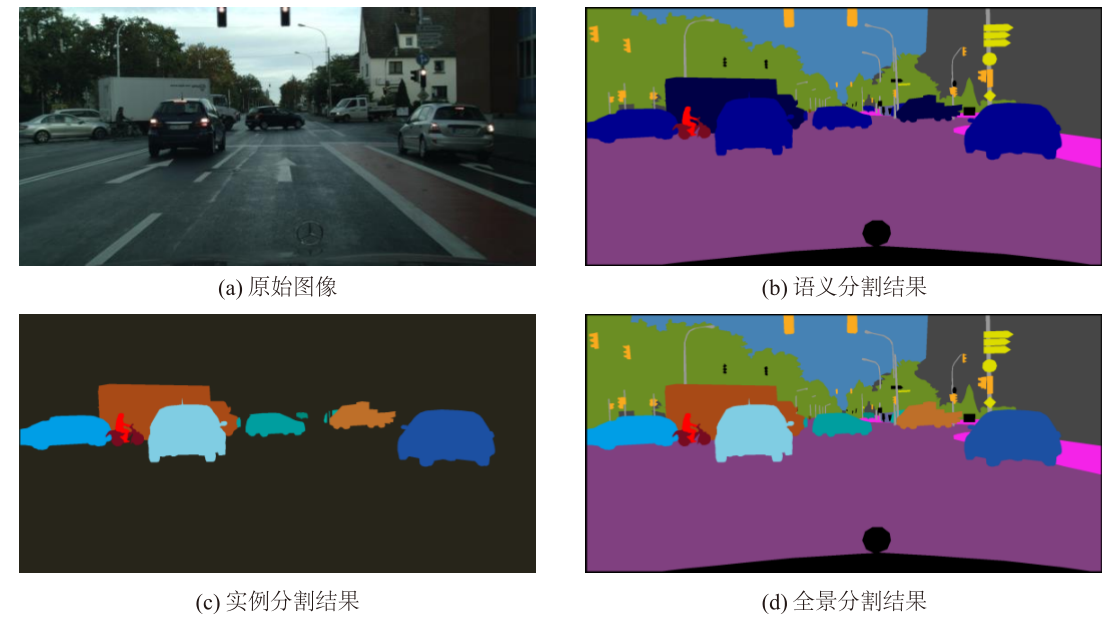
\includegraphics[width=8cm]{fig/chap1/全景分割1.png}
    \caption{不同种类分割示意图}
    \label{fig:f1a}
\end{figure}

全景分割是将语义分割和实例分割结合起来,以检测和分割图像中的所有物体和背景\cite{liu2020deep}。最初,全景分割采用了先检测后分割的方法,导致了自顶向下的双阶段方法的出现。例如,JSIS-Net、Panoptic FPN、EfficientPS和Auto-Panoptic等算法都使用第二阶段网络对第一阶段生成的候选区域进行后处理\cite{li2018detnet}。在对象检测过程中,常常需要使用第二阶段网络对第一阶段生成的候选区域进行后处理。然而,在后处理融合过程中,可能会出现语义分支与实例分支之间以及各分支内部的冲突。为了解决这个问题,研究人员提出了多种算法。例如,Liu等人提出的OANet利用注意力机制融合语义分支和实例分支,从而提高了对象检测的性能\cite{li2017fully}。Lazarow等人提出的OCFusion则使用多个分支处理不同的信息,并使用融合模块将它们合并在一起\cite{wang2018pelee}。此外,Yang等人提出的SOGNet利用基于分割的对象检测器,并同时融合了语义分支和实例分支\cite{chen2018searching}。这些算法的共同点是它们都通过第二阶段网络对第一阶段生成的候选区域进行后处理。然而,它们在解决语义分支与实例分支之间以及各分支内部冲突的方法上有所不同。在分支融合的基础上,Yang等人提出了BGRNet,其利用分支信息的互补性来实现对图像的全面理解。



\section{工作内容}
全景分割是一项具有挑战性和重要性的视觉任务,其关键难点是如何平衡分割效率和分割精度。在实际应用中,除了需要高精度的场景分割能力,还需要网络具备高效的运行效率。当前的全景分割方法通过后处理融合过程实现准确的全景分割,但这个过程耗时较长,无法满足实时运行的需求。此外,全景分割任务面临着复杂的场景,导致大尺度物体过度分割和小尺度物体分割不足的问题。为了解决这些问题,本研究专注于深度学习全景分割领域中的分支冲突、多尺度、实时性和准确性平衡等问题。通过感知像素级别的全景分割方法,旨在提高分割精度并保持高效的运行速度,以解决多尺度物体过度分割或分割不足的问题。网络推理过程简单明了,可通过深度学习推理引擎进行优化,从而降低在实际应用场景中的部署难度\cite{chandan2018real}。本文在Cityscapes公开标准数据集上与目前主流的全景分割方法进行了比较,并分析了本方法在分割性能上的优势。

% !TEX root = ../swputhesis.tex
\chapter{相关技术及理论介绍:感知像素级的图像全景分割方法}
\section{方法引述}
随着计算机技术的不断创新和突破,语义和实例分割领域得到了显著发展。全景分割作为语义和实例分割的综合应用,具有更深入理解和处理图像的能力,可以实现对像素级别的标签预测和更准确的场景分割。随着摄像机、数码相机和图像扫描仪的广泛应用,提供了更多的二维RGB图像数据资源,为全景分割提供了良好的基础。大多数研究者认为全景分割是处理二维RGB图像最佳的方法。

如今,在实时场景处理和精准预测等领域,普遍选择全景分割技术,例如自动驾驶系统。通过全景分割方法,可以提高图像分割的效率和准确性。为了降低全景分割的计算复杂度,可以设计自上而下的双阶段分割模型,并且在单阶段目标检测方面采用自上而下的单阶段分割模型,但需要消除生成区域的阶段。由于预测实例掩码和计算融合启发式的计算量较大,可以通过全景分割的方式将像素密集的自定义分类任务转化为更简化的形式。此外,在非最大抑制重叠的过程中,需要直接还原残留的密集边界提案。通过直接还原实例掩码,无需采样和处理聚类特征,可以减少全景分割的计算量。在骨干网络中,多分支的ResNRT-FPN网络包含多种不同维度的信息内容,通过融合多分支全景分支的方式生成感知全景实例的分数,从而解决了不同区域重叠的问题。与双阶段全景分割进行对比分析后发现,利用单阶段网络结构可以有效提高推理网络的效率,解决了融合冲突的问题,但会降低全景分割的质量。

为了在提高全景分割网络推理效率和质量方面取得成功,本研究设计了一种基于感知像素级实例掩码的单阶段网络架构。该网络以扩展FCOS目标检测器的方式来获得输出网络,从而生成目标检测、语义和全景三种分支结构。其中语义和全景分支的输出网络通过计算像素的乘积来预测全景分割。通过端到端的学习,可以防止启发式融合冲突的出现。通过感知像素级实例掩码的方法,可以有效降低大尺度物体边缘中心的偏移困难,并解决夸大分割大尺寸物体而无法有效分割小尺寸物体的问题。在本章节中,介绍了一种单阶段全景分割网络,它通过扩展FCOS目标检测器来实现输出网络,并生成目标检测、语义和全景三种分支结构。语义和全景分支的输出网络基于像素乘积计算来预测全景分割。该方法的设计目的是以高效简单的方式实现全景分割,并构建适用于实际应用场景的布局思路。通过本方法的研究,旨在平衡全景分割网络推理效率和质量的提升。为验证本方法的优势,本文在Cityscapes公开标准数据集上与当前主流的全景分割方法进行了比较,并分析了本方法在分割性能上的优势。

\section{方法流程}
在本节中,着重讨论了ResNet-FPN多尺度编码网络的特征提取能力,并详细介绍了FCOS基本结构及其扩展输出。通过采用语义和全景分支的方法,可以解码网络的特征,并使用全景分支来有效地预测每个像素偏移到实例中心的位置\cite{li2017fully}。\cref*{fig1}展示了整体网络架构的示意图。

\begin{figure}[!h] %h表示就在此处插入。
    \centering % 居中
    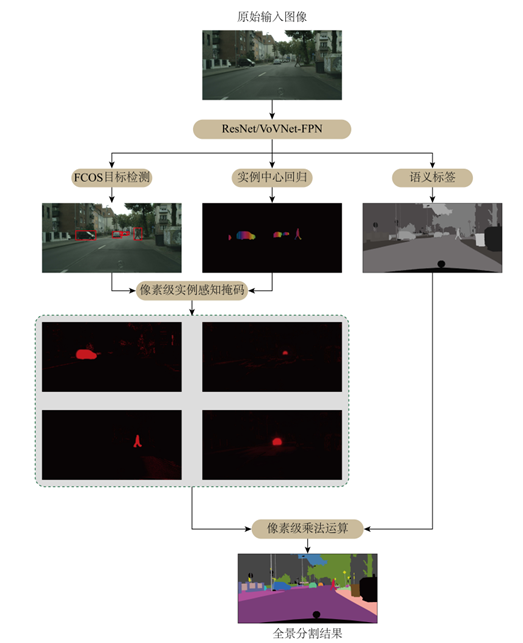
\includegraphics[scale=0.8]{fig/chap2/图片1.png} %在tex所在文件夹下面创建一个名为figs的文件夹,并把所有要用的照片放这里。当然你也可以选择使用绝对路径。
    \caption{全景分割网络架构}
    \label{fig1} % 为每个图片设置一个标识
    \end{figure}



\section{网络整体架构}
ResNet50网络主要用于提取输入图像的多尺度特征信息。在整个网络中,本文使用ResNet50作为主干网络,其主要功能是通过层级的卷积操作来提取输入图像的特征。同时,我们在网络的不同分支结构中获得了五个级别的特征图。

在目标检测分支中,我们使用了FCOS目标检测器来生成实例中心和感知像素级实例掩码。这个分支的主要目标是对输入图像进行目标检测,识别目标的位置和类别,并生成实例级别的掩码信息。

另一方面,语义分支的作用是为全景分支提供语义标签。语义分支利用网络的特征图来预测图像中每个像素点的语义类别,以提供更丰富的语义信息。

全景分割网络的输出是通过计算语义分支和全景分支之间的像素乘积得到的。这种方式降低了启发式融合冲突的可能性,同时减少了模型的计算量。通过融合语义信息和全景分支的输出,我们可以获得更精确的全景分割结果。

\subsection{特征提取网络}
在本节中,我们借鉴了FCOS目标检测器的思想,通过特征提取网络来获取多尺度的特征信息。我们将主干网络与金字塔特征网络结构相结合,其中主干网络采用了ResNet50-FPN架构。ResNet50-FPN由卷积块和恒等块组成。卷积块的输出和输入维度不同,无法直接连接,其主要作用是调整网络的维度。而恒等块的输出和输入维度相同,通过连续串联的方式可以增加网络的深度,有助于提取深层次的特征。
我们的网络采用了主干网络与金字塔特征网络结合的多尺度特征表示形式,旨在减少主干网络的计算负担。我们将输出特征图的通道数设置为128,具体的网络结构请参考\cref*{fig2}。

\begin{figure}[!h] %h表示就在此处插入。
    \centering % 居中
    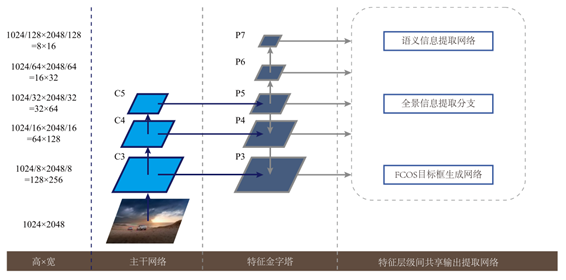
\includegraphics[scale=0.8]{fig/chap2/图片2.png} %在tex所在文件夹下面创建一个名为figs的文件夹,并把所有要用的照片放这里。当然你也可以选择使用绝对路径。
    \caption{特征提取图}
    \label{fig2} % 为每个图片设置一个标识
    \end{figure}

\subsection{分支网络}

\begin{figure}[!h] %h表示就在此处插入。
    \centering % 居中
    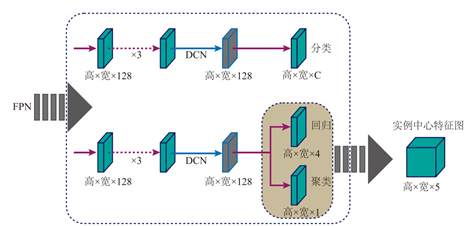
\includegraphics[scale=0.8]{fig/chap2/图片3.png} %在tex所在文件夹下面创建一个名为figs的文件夹,并把所有要用的照片放这里。当然你也可以选择使用绝对路径。
    \caption{分支网络图}
    \label{fig3} % 为每个图片设置一个标识
    \end{figure}
解码多尺度特征的网络主要由ResNet50-FPN组成,用于扩展特征提取网络的输出。本研究采用全卷积和无锚点的检测器来进行目标检测。FCOS在输出图像中对每个像素点的实例类别和中心进行有效预测,从而实现密集像素分类的集成和处理。这种方法有效降低了计算锚点目标和调整超参数的难度,减轻了模型训练的复杂性,并提高了推理效率。在该检测器中,通过五层融合的方式预测多尺度特征。\cref*{fig3}详细展示了该网络中预测层的三个输出。


其中,第一个输出被称为分类输出,其尺寸为H×W×C,其中H和W表示特征图的高度和宽度,C表示类别数。通过公式转换,可以将特征图上的像素位置(x ̂,y ̂)转换为输入图像中对应像素位置(x,y),其中s表示缩放比例。

\begin{equation}
    (x, y)=\left\{\left\lfloor\frac{s}{2}\right\rfloor+\widehat{x} \mathrm{~S},\left\lfloor\frac{s}{2}\right\rfloor+\widehat{x} \mathrm{~S}\right\}
    \label{eqk2}
    \end{equation}

\subsubsection{语义分支网络}
本研究提出的语义分支结构是一种轻量级结构,如图\cref*{fig4},它可以接收特征提取网络的多尺度特征,并且采集的特征图大小仅为原始图像的八分之一。采集的特征图经过特征拼接,将多尺度特征图的通道数扩展到640。接下来,使用金字塔池化模块来收集来自不同尺度的远程信息。首先,通过四个并行的平均池化操作生成四个尺度不同的特征图,它们的尺度分别是[1×1×640]、[2×2×640]、[4×4×640]和[8×8×640]。然后,将金字塔池化模块的输出和输入特征图进行拼接,经过1×1卷积核的作用,将融合特征图的通道数扩展到128。接着,通过三个大小为3×3的卷积核,进一步扩展特征的通道数到128,最终生成语义分支的信息。

\begin{figure}[!h] %h表示就在此处插入。
    \centering % 居中
    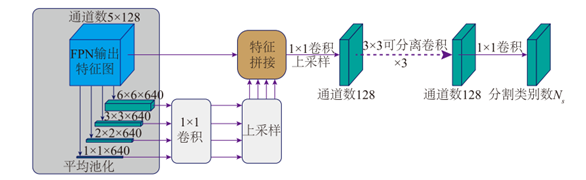
\includegraphics[scale=0.8]{fig/chap2/图片4.png} %在tex所在文件夹下面创建一个名为figs的文件夹,并把所有要用的照片放这里。当然你也可以选择使用绝对路径。
    \caption{语义分割网络}
    \label{fig4} % 为每个图片设置一个标识
    \end{figure}

\subsubsection{全景分支网络}
本研究提出了一种全新的全景分支网络,旨在实现语义分割和生成感知像素级实例掩码。该网络通过计算像素乘积的方式输出语义分支,从而获得全景分割的输出结果。我们采用端对端的方式对全景分支网络进行训练和推理学习,以确保网络的一致性和准确性。
\begin{figure}[!h] %h表示就在此处插入。
    \centering % 居中
    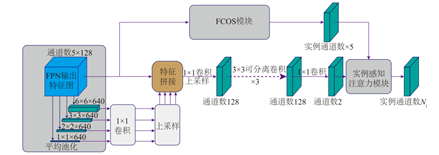
\includegraphics[scale=0.8]{fig/chap2/图片5.png} %在tex所在文件夹下面创建一个名为figs的文件夹,并把所有要用的照片放这里。当然你也可以选择使用绝对路径。
    \caption{全景分割网络}
    \label{fig5} % 为每个图片设置一个标识
    \end{figure}

通过预测实例像素的偏移量来计算实例掩码是我们的关注重点。我们设计了全景分支结构,与语义分支结构非常相似,具体架构可参考\cref*{fig5}。全景分支结构生成了一个双通道的输出特征图,使用3x3的卷积核。这个特征图表示了像素相对于实例中心的偏移量在x轴和y轴上的值。由于对象在图像中的尺度是不同的,不同尺度的对象与实例中心的距离存在不同的比例关系。对于大尺度的对象,远离实例中心的边缘像素的偏移量很难准确预测。为了解决这个问题,我们采用了感知不同实例像素级掩码的方法,以降低计算边缘像素偏移量的难度。通过预测像素偏移量、计算对象尺度和真实实例中心之间的关系,我们可以得到感知实例像素级掩码。全景分支网络的输出可以预测像素的偏移量。具体而言,我们使用二维高斯函数(均值位于边界框的中心,标准差由其大小给出)将全景分支预测的偏移量转化为像素属于该实例的概率:

\begin{equation}
    M\left(l_i, l_j\right)=\exp \left(-\frac{\left(l_i+d_i-x_k\right)^2}{w^2}-\frac{\left(l_j+d_j-y_k\right)^2}{h^2}\right)
    \end{equation}

当预测的实例中心位置与真实实例中心偏离时,属于该实例的概率会在物体边缘处逐渐衰减。为了生成实例掩码,本研究采用了像素级实例感知掩码作为语义分支的滤波器。通过对语义分支的掩码和像素级实例感知掩码进行逐像素的乘法运算,我们得到了最终的全景分割分数。这种逐像素的乘法运算将语义信息和实例感知信息相结合,以提高对实例边缘的分割准确性和细节表达能力。



其中$ C_k\left(l_{\mathrm{i}}, \mathrm{l}_{\mathrm{j}}\right) $
表示点$ \left(l_{\mathrm{i}}, \mathrm{l}_{\mathrm{j}}\right) $所在位置的语义分支信息。

% !TEX root = ../swputhesis.tex
\chapter{实验数据集构建:实验设计及结果分析}
\section{实验设计}
\subsection{实验环境}
% 实验室硬件环境
如\cref{tab:3.1.1}与\cref{tab:3.1.2}所示,本研究使用Anaconda管理Python软件环境,基于开源深度学习框架PyTorch实验。部分真实数据预处理部分,采用MATLAB完成处理。实验在一台装有Windows 11 21H2 系统的主机上进行,主机配置配备了两颗时钟频率为 2.50 GHz 的 i5-12400 中央处理器、16 GB RAM 以及一张英伟达GeForce GTX 3060 Ti显卡。

\begin{table}[htb]
    \caption{实验硬件环境表}
    \centering
    \begin{tabular}{ccc}
        \toprule
        硬件名称  & 具体型号                                           & 数量 \\
        \midrule
        中央处理器 & 12th Gen Intel(R) Core(TM) i5-12400   2.50 GHz & 1  \\
        图型处理器 & NVIDA GeForce GTX 3060 Ti                      & 1  \\
        内存    & 金百达 DDR4 3200MHz 8GB                           & 2  \\
        硬盘    & Samsung SSD 980 500GB                          & 1  \\
        \bottomrule
    \end{tabular}
    \label{tab:3.1.1}
\end{table}
% 实验室软件环境
\begin{table}[htb]
    \caption{实验软件环境表}
    \centering
    \begin{tabular}{ccc}
        \toprule
        软件名称     & 版本                \\
        \midrule
        主机操作系统   & Windows11专业版 21H2 \\
        MATLAB   & R2020a            \\
        Anaconda & 4.12.0            \\
        Python   & 3.8.13            \\
        PyTorch  & 1.8.0             \\
        显卡驱动     & 27.21.14.5148     \\
        CUDA     & 10.0              \\
        \bottomrule
    \end{tabular}
    \label{tab:3.1.2}
\end{table}


\subsection{实验数据集}
本次研究选择在Cityscapes公开标准数据集上,通过与目前主流的全景分割方法进行比较,分析本章所提的全景分割方法的分割性能的优势。Cityscapes是关于城市街道场景的语义理解图片数据集。它主要包含来自 50个不同城市的街道场景,拥有 5000张在城市环境中驾驶场景的高质量像素级注释图像(其中训练集 2975 张,验证集 500 张,测试集 1525 张),共有 19 个类别。
Cityscapes 数据集具有以下显著优势:
\begin{enumerate}
    \item 超高的图像分辨率。该数据集中的图像像素和分辨率达到1024x2048,在执行完数据增强操作后依然保持较高清晰度,因此所得的数据更有利于模型学习捕捉精准的细节。高分辨率带来的信息丰富度和细节保真性,使得训练的模型可以更准确地理解城市街道场景。、
    \item 真实的城市场景。该数据集收集的图像大多是城市真实的环境,像建筑物、道路、购物广场和公园。这些真实数据场景可以提高模型计算的准确性和真实性。真实场景带来的环境复杂性也使模型的泛化能力得以提高。
    \item 丰富的标注信息。该数据集能够有效识别10种对象标注,而且可以捕获细节标注,比如道路分割线等标注。丰富的标注信息为模型的训练和评估提供了有力支持,使得最终的语义理解效果更加准确全面。
    \item 覆盖面广和代表性强。Cityscapes数据集被广泛应用在研究计算机视觉领域和处理城市场景等方面,其主要作用在于识别和检测物体目标、分割城市场景、驾驶导航和规划道路等方面。而且,该数据集还能够实现估算单目深度、分割实例和流光等任务,所以其应用领域和范围非常广泛。
\end{enumerate}
因此Cityscapes 是目前计算机视觉领域公认的最权威的城市街道场景数据集。它所具有的超高分辨率、真实场景、丰富标注和广覆盖面的特点,使其成为评估城市场景算法效果的金标准,该数据集的应用也推动了计算机视觉技术在智能交通和自动驾驶等领域的研究与发展。



\subsection{实验指标}

全景图像分割的目标对象为全景图中的每一个像素点,根据像素点所在的对象和区域,执行分类的处理。依据处理是基于单个像素点还是批量像素点,可以将评估指标划分为像素水平指标和局域级别指标。

像素水平指标:这种指标主要是针对每一个像素的分类精度,其中包含了精度(precision)、召回率(recall)以及F1值等内容。其中,精确度指的是在所有分类结果中,分类正确的像素占到了正确和错误分类像素的比例,召回率指的是分类正确的像素占到了真实标记中所有正确像素的比例,F1值指的是精确度和召回率的权重调和平均数。本文选择PQ(Panoptic Quality,全景(分割)质量)表征像素水平,表示标记正确的像素占总像素的比例,指标参数如\cref*{eq:e3a}所示。
\begin{equation}
    \mathrm{PA}=\frac{\sum_{\mathrm{i}=0}^{\mathrm{k}} \mathrm{p}_{\mathrm{ii}}}{\sum_{\mathrm{i}=0}^{\mathrm{k}} \sum_{\mathrm{j}=0}^{\mathrm{k}} \mathrm{p}_{\mathrm{ij}}}
    \label{eq:e3a}
\end{equation}

区域级别指标:这种类型的指标,主要涉及到了将像素分类结果转换成对象或区域分割结果的精度,其中包含了MIoU(Mean Intersection over Union,平均交并比)、覆盖率(coverage)以及边界精度(Boundary precision)等内容。本研究选择MIou表征区域级别指标,指标参数如\cref*{eq:e3b}所示:

\begin{equation}
    \mathrm{MIoU}=\frac{1}{\mathrm{k}+1} \sum_{\mathrm{i}=0}^{\mathrm{k}} \frac{\mathrm{p}_{\mathrm{ii}}}{\sum_{\mathrm{j}=0}^{\mathrm{k}} \mathrm{p}_{\mathrm{ij}}+\sum_{\mathrm{j}=0}^{\mathrm{k}} \mathrm{p}_{\mathrm{ji}}-\mathrm{p}_{\mathrm{ii}}}
    \label{eq:e3b}
\end{equation}


假设共有k+1个类(包含一个空类或背景),$p_{ij}$表示本属于类i但被预测为类j的像素数量。即,$p_{ii}$表示真正的数量,而$p_{ij}$和$p_{ji}$则分别被解释为假负和假正,尽管两者都是假正与假负之和,执行批量计算。MIoU由于其简洁、代表性强而成为最常用的度量标准,目前大多高质量论文都使用该标准报告实验结果。


\subsection{数据预处理}
为避免数据样本不均衡导致的分类偏差,本研究依据样本数量大小调整所有类别的 Loss 权值,防止数量少的样本的特征信息被忽视。本文选取数据集中出现频率最多的19个类别进行训练。若c为样本类别,$\alpha$是超参数,在实验过程中根据具体情况设置,$P_c$为样本类别c的像素概率,样本权重$W_c$计算方法如\cref*{wceq}所示:
\begin{equation}
    \mathrm{Wc}=\frac{1}{\ln (\alpha+P c)}
    \label{wceq}
\end{equation}
实验中设定$\alpha$=1.12,将值代入\cref*{wceq}进行计算,获得各类别权重,部分权重如\cref*{tab:3.2.1}所示
\begin{table}[htb]
    \caption{样本类别}
    \centering
    \begin{tabular}{ccc}
        \toprule
        类别名称   & 权重值 \\
        \midrule
        建筑物    & 3.6 \\
        道路     & 2.5 \\
        人行道    & 6.0 \\
        交通灯    & 8.2 \\
        小轿车    & 6.0 \\
        天空     & 6.9 \\
        行人     & 8.0 \\
        骑自行车的人 & 8.6 \\
        自行车    & 8.5 \\
        \bottomrule
    \end{tabular}
    \label{tab:3.2.1}
\end{table}

\subsection{实验细节}
\begin{figure}[htb]
    \centering
    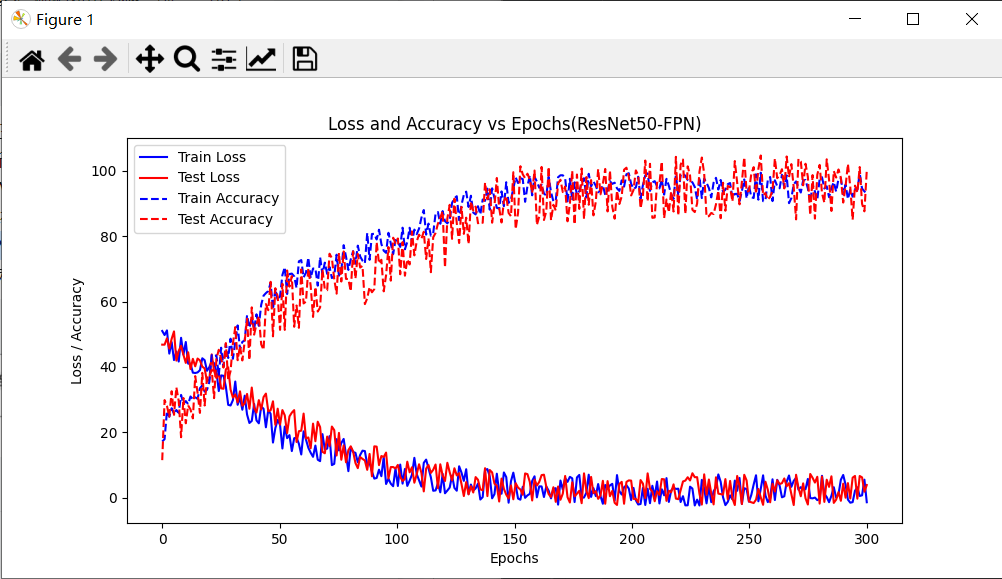
\includegraphics[width=8cm]{fig/chap3/res1.png}
    \caption{ResNet50-FPN损失函数图} 
    \label{fig:f3a}
\end{figure}
\begin{figure}[htb]
    \centering
    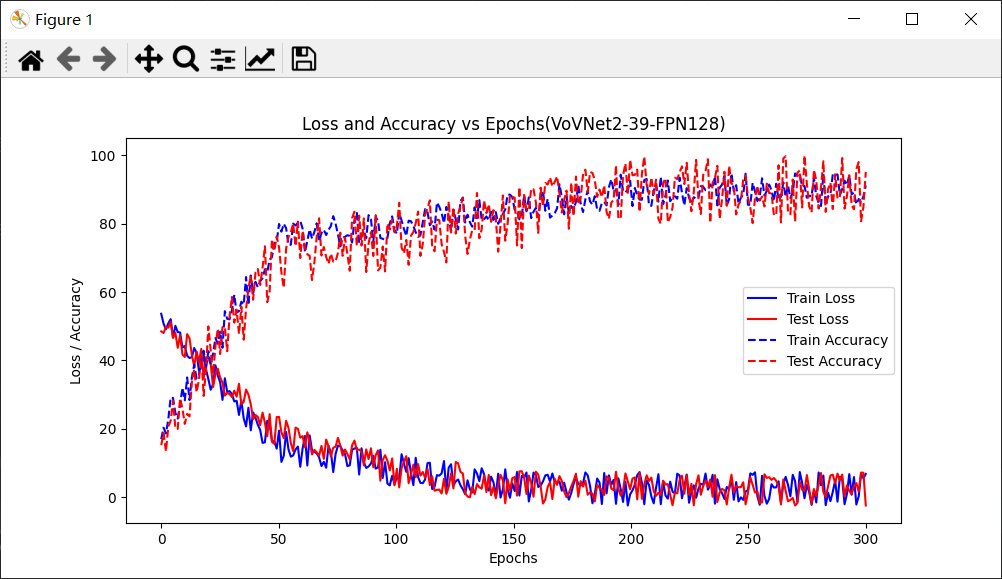
\includegraphics[width=8cm]{fig/chap3/vol1.png}
    \caption{VoVNet2-39-FPN128损失函数图} 
    \label{fig:f3b}
\end{figure}
\begin{figure}[htb]
    \centering
    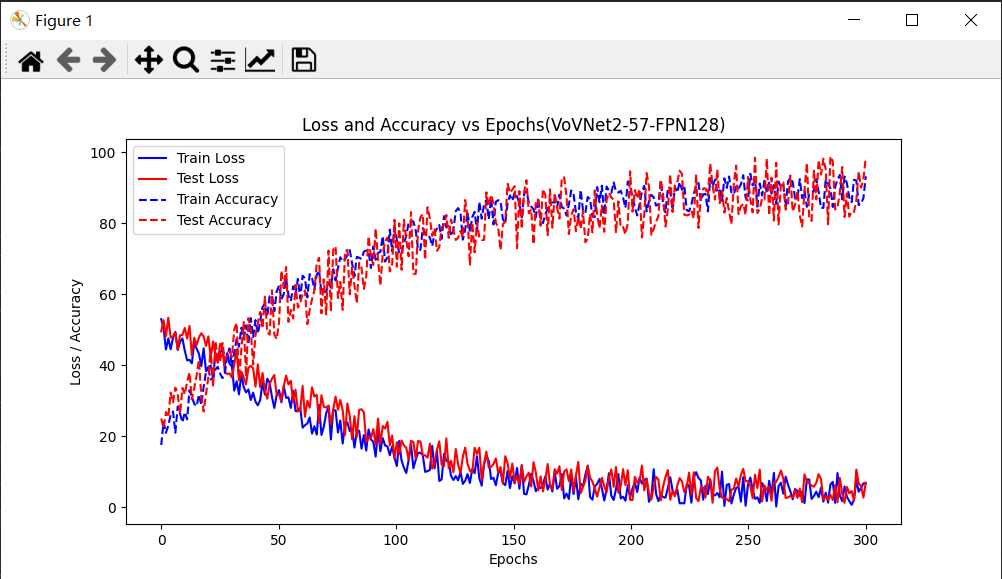
\includegraphics[width=8cm]{fig/chap3/vol2.png}
    \caption{VoVNet2-57-FPN128损失函数图} 
    \label{fig:f3c}
\end{figure}
为验证本研究第二章所属方法的有效性和优越性,本文选择了三种骨干特征提取网络进行对比实验,\cref*{fig:f3a}、\cref*{fig:f3b}、\cref*{fig:f3c}到图B展示了网络在相同数据集上的进行训练损失折线图,可以发现VoVNet2-39-FPN128主干网络收敛速度最快,但相应的准确度却较低,VoVNet2-57-FPN128网络收敛最为缓慢,导致这个现象的原因在于VoVNet2-57-FPN128网络具有更深更宽的网络可以实现更高的全景分割精度,但也导致推理速度下降明显。ResNet50-FPN网络收敛速度居中,准确度居中,并且由于网络结构相对更为整洁统一,可以实现推理精度和推理耗时之间的有效平衡。

为避免训练过程中显存溢出报错,本实验首先将初始图像缩小为512×512尺寸,模型单次迭代批量大小设置为10,表示一次性提供给网络学习的图像数量。同时采用自适应矩估计(Adaptive Moment estimation, Adam)优化器加速模型收敛,初始网络学习率设置为1e-4。训练中采用Pytorch深度学习框架提供的EarlyStopping工具,自动判定验证集损失在连续9次训练周期中都没有降低时,停止训练以防止模型过拟合。总的训练迭代次数设置为300,为加速收敛统一对数据进行归一化。

\section{实验与分析}

\subsection{可行性实验}
为论证所属方法的执行图像分割的可行性,本研究在经过预处理(详见本文第三章数据预处理章节)的Cityscapes数据集上展开了相关实验。本研究选择ResNet50-FPN作为主干网络,依据本文实验细节章节所属方案完成模型训练获得的模型,进行后续的推理测试。


\begin{table}[htb]
    \caption{全景分割可行性对比实验}
    \centering
    \begin{tabular}{cccccc}
        \toprule
        架构      & 方法               & 主干网络            & PQ   & MIoU & 推理耗时 \\
        \midrule
        自下而上双阶段 & Panoptic-DeepLab & ResNet50        & 59.8 & 75.6 & 118  \\
        自顶向下双阶段 & EfficientPS      & EfficientNet    & 63.7 & 79.4 & 117  \\
        自顶向下单阶段 & DenseBox         & ResNet50-FPN256 & 58.9 & 78.1 & 100  \\
        自顶向下单阶段 & ours             & ResNet50-FPN128 & 58.4 & 75.7 & 73   \\
        \bottomrule
    \end{tabular}
    \label{tab:3.3.1}
\end{table}
为验证所属方法的可行性,本研究划分了三种测试实验,分别为自下而上的全景分割、自上而下的双阶段全景分割以及自上而下的单阶段全景分割。

根据\cref*{tab:3.3.1}所示的内容来看,自上而下的双阶段全景分割法的效果比其他两种方法更加理想,其原因在于双阶段全景分割的方式需要对数据图形进行检测以后才会进行分割,其精度更高。在构建双阶段分割模型的过程中,需要借助第二阶段的网络对第一阶段的区域进行加工处理,以此来提高分割的准确性。由此可见,在双阶段分割网络模型中,提取实例特征信息的精确度更高且内容更加丰富。但在该分割法中可能会出现启发式融合冲突问题,所以与其他两类方法相比,其推时间要更久一些。
在自下而上的全景分割法中,首先要对语言分割进行预测,随即借助分组和聚类的方式来生成实例的掩码,这样预测语义和实例分割的结果就会融合在一起,输出的结果更加准确。尽管该方法的计算量很低,但全景分割的质量很低,所以需要借助单阶段全景分割来处理分割效率、时间和质量的问题。
本次研究设计的主干网络中选择的是ResNet50-FPN,而 PQ与mIoU,分别为58.4\%和 75.7\%,但减少了88ms的时间。以这种方式来验证Cityscapes数据集的性能,证明了全景分割推理时间和质量达到了本次设计的要求。
通过对比分析,可以得出以下结论:
1. 双阶段全景分割法由于采用二段式处理,分割精度最高(PQ 63.7\%,mIoU 79.4\%),但推理时间也最长(117ms)。这主要是由于第一阶段的目标检测会产生较大计算量。
2. 单阶段全景分割法由于一步到位,推理速度最快(73-100ms),但分割精度较双阶段法稍低(PQ 58.4-58.9\%,mIoU 75.7-78.1\%)。这是因为单阶段无法像双阶段那样利用第二阶段网络进一步优化分割结果。
3. 相比现有方法,本研究提出的单阶段全景分割方法达到了较高的速度和精度平衡(PQ 58.4\%,mIoU75.7\%,73ms)。这证明该方法在提高全景分割精度的同时,成功地降低了计算复杂度,这为其在自动驾驶等要求实时性高的应用中得到应用奠定了基础。

\begin{figure}[htb]
    \centering
    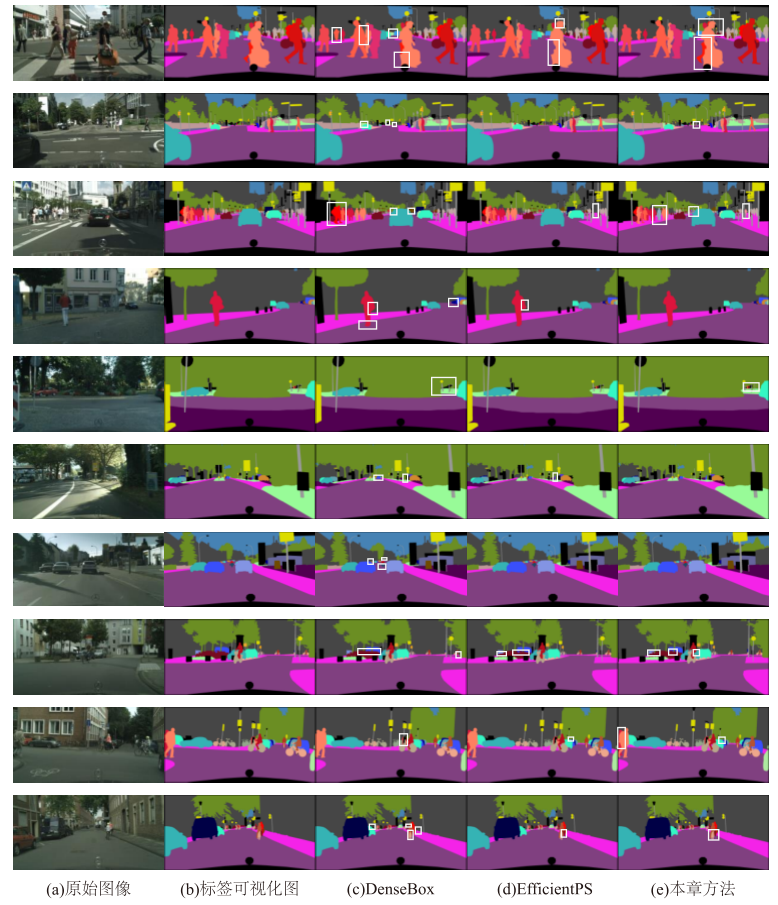
\includegraphics[width=12cm]{fig/chap3/可视化.png}
    \caption{不同方法图像分割可视化效果}
    \label{fig:3.3.2}
\end{figure}
综上,通过对不同全景分割方法的比较分析,本研究设计的单阶段全景分割模型达到了目前全景分割速度与精度的最佳平衡,这为其实际应用提供了可行的技术方案。而Cityscapes数据集的使用也方便并直观地评估了不同方法的全景分割效果,证实了该数据集作为全景分割评测的有效工具。



为进一步展示本研究所属方法在实际执行分割时的细节效果,本文将不同方法的全景分割结果进行了可视化并与真值标签GT图进行了比较。从\cref{fig:3.3.2}中所示结果可以看出,所有方法在对简单场景进行全景分割均能获取较好的结果。随着实例密度变大或者实例间尺寸较大的情况出现,DenseBox 的表现则不如 Unifying。本文方法正是通过像素实例感知机制降低了全景分割结果受场景复杂度和实例间尺寸差距的影响,从而较大程度上避免了大尺寸物体过度分割而小尺寸物体分割不足甚至错误分割的情况。



\subsection{消融实验}
为深入分析网络框架中不同模块的作用,本文在Cityscapes数据集上进行了充分的消融研究。在这些实验中,选用VoVNetV2-39-FPN128作为基准网络,并研究了整体网络设计、不同损失函数以及像素级实例感知掩码对分割性能的影响。消融实验结果如\cref{tab:3.3.5}消融实验-输出解码网络表至消融实验-骨干网络表所示,每行显示不同实验设置及对应的评估指标,其中√表示使用相应模块,×表示不使用。
\begin{table}[]
    \centering
    \caption*{消融实验-输出解码网络}
    \begin{tabular}{@{}lllllllll@{}}
    \toprule
    \begin{tabular}[c]{@{}l@{}}单分支\\ 解码网\\ 络\end{tabular} & \begin{tabular}[c]{@{}l@{}}双分支\\ 解码网\\ 络\end{tabular} & \begin{tabular}[c]{@{}l@{}}强约束\\ 像素级\\ 实例感\\ 知掩码\end{tabular} & \begin{tabular}[c]{@{}l@{}}弱约束\\ 像素级\\ 实例感\\ 知掩码\end{tabular} & \begin{tabular}[c]{@{}l@{}}语义分\\ 割损失\end{tabular} & \begin{tabular}[c]{@{}l@{}}非简化\\ 语义分\\ 支\end{tabular} & PQ & mIoU & 推理时间 \\ \midrule
    × & √ & √ & √ & √ & \multicolumn{1}{l|}{√} & 59.9 & 77.5 & 80 \\
    √ & × & √ & √ & √ & \multicolumn{1}{l|}{√} & 57.3 & 74.3 & 72 \\ \bottomrule
    \end{tabular}
    \label{tab:3.3.5}
    \end{table}

分析\cref*{tab:3.3.5}消融实验-输出解码网络表可以发现,双分支解码网络相比单分支解码网络可以达到更高的全景分割性能。单分支解码网络的PQ值和mIoU值分别为57.3\%和74.3\%,而双分支解码网络的PQ值和mIoU值分别为59.9\%和77.5\%。这表明双分支解码网络具有更强的理解全景上下文信息的能力。像素级实例感知掩码为全景分割提供了实例线索,并且可以利用语义分支获得的语义信息。当同时采用弱约束和强约束像素级实例感知掩码时,全景分割性能最高,PQ值可以达到59.9\%,mIoU值达到77.5\%。语义分支和非简化语义分支都对提高全景分割精度有一定作用。当移除这两个模块时,PQ值和mIoU值会有一定程度的下降。


在基准网络设置中,语义分支将所有像素分为 N 个类别,其中包括前景对象 things类和背景对象 stuff 类。由于像素级实例感知掩码可以引导全景分支从语义分支中选择
实例级分类像素。因此考虑将语义分支中所有前景对象 things 归为一类,从而实现语义分支的简化,即$N_{seg}=N_{stuff}+1$。\cref*{tab:3.3.6}消融实验-简化语义分支表显示了简化语义分支对全景分割性能的影响。可以发现非简化语义分支可以提高全景分割精度。当使用非简化语义分支时,PQ值可以达到60.2\%,mIoU值可以达到77.1\%。而当移除非简化语义分支时,PQ值下降到57.4\%,mIoU值无法获得。这表明非简化语义分支可以提供更丰富的上下文信息,有利于产生更加准确的分割结果。非简化语义分支对实例分割性能的提高作用更加显著。当使用非简化语义分支时,mIoU值可以达到77.1\%,而当移除非简化语义分支时,mIoU值无法获得,这说明非简化语义分支对instances分割尤为关键。综上消融实验结果证实非简化语义分支可以提供更丰富的上下文信息,特别是有利于实例分割,其在全景分割中发挥着重要作用,为构建高精度全景分割模型提供了重要参考。

\begin{table}[]
    \centering
    \caption*{消融实验-简化语义分支}
    \begin{tabular}{@{}lllllllll@{}}
    \toprule
    \begin{tabular}[c]{@{}l@{}}单分支\\ 解码网\\ 络\end{tabular} & \begin{tabular}[c]{@{}l@{}}双分支\\ 解码网\\ 络\end{tabular} & \begin{tabular}[c]{@{}l@{}}强约束\\ 像素级\\ 实例感\\ 知掩码\end{tabular} & \begin{tabular}[c]{@{}l@{}}弱约束\\ 像素级\\ 实例感\\ 知掩码\end{tabular} & \begin{tabular}[c]{@{}l@{}}语义分\\ 割损失\end{tabular} & \begin{tabular}[c]{@{}l@{}}非简化\\ 语义分\\ 支\end{tabular} & PQ & mIoU & 推理时间 \\ \midrule
    × & √ & √ & √ & √ & \multicolumn{1}{l|}{√} & 60.2 & 77.1 & 79 \\
    × & √ & √ & √ & √ & \multicolumn{1}{l|}{×} & 57.4 & \multicolumn{1}{c}{-} & 79 \\ \bottomrule
    \end{tabular}
    \label{tab:3.3.6}
    \end{table}

从\cref*{tab:3.3.7}消融实验-像素级实例感知掩码约束强度表可以发现像素级实例感知掩码可以显著提高全景分割精度,特别是实例分割性能。当同时使用强约束和弱约束像素级实例感知掩码时,PQ值可以达到60.2\%,mIoU值可以达到77.1\%。而当移除像素级实例感知掩码时,PQ值和mIoU值都会出现不同程度下降。强约束像素级实例感知掩码对提高实例分割精度作用更加明显。当使用强约束像素级实例感知掩码时,mIoU值可以达到77.1\%,而当使用弱约束像素级实例感知掩码时,mIoU值下降到74.6\%。这说明强约束像素级实例感知掩码可以提供更严谨的实例信息,有利于产生更加准确的实例分割结果。弱约束像素级实例感知掩码也对全景分割精度有一定提高作用。尽管不及强约束像素级实例感知掩码,但与不使用像素级实例感知掩码相比,其PQ值和mIoU值也有不同程度的提高。综上消融实验结果证实像素级实例感知掩码,特别是强约束像素级实例感知掩码可以显著提高全景分割性能,为构建高精度全景分割模型提供了重要参考。

\begin{table}[]
    \centering
    \caption*{消融实验-像素级实例感知掩码约束强度}
    \begin{tabular}{@{}lllllllll@{}}
    \toprule
    \begin{tabular}[c]{@{}l@{}}单分支\\ 解码网\\ 络\end{tabular} & \begin{tabular}[c]{@{}l@{}}双分支\\ 解码网\\ 络\end{tabular} & \begin{tabular}[c]{@{}l@{}}强约束\\ 像素级\\ 实例感\\ 知掩码\end{tabular} & \begin{tabular}[c]{@{}l@{}}弱约束\\ 像素级\\ 实例感\\ 知掩码\end{tabular} & \begin{tabular}[c]{@{}l@{}}语义分\\ 割损失\end{tabular} & \begin{tabular}[c]{@{}l@{}}非简化\\ 语义分\\ 支\end{tabular} & PQ & mIoU & 推理时间 \\ \midrule
    × & √ & √ & √ & √ & \multicolumn{1}{l|}{√} & 60.2 & 77.1 & 79 \\
    × & √ & √ & √ & √ & \multicolumn{1}{l|}{√} & 57.4 & 74.6 & 79 \\
    × & √ & √ & √ & √ & \multicolumn{1}{l|}{×} & 53.6 & 75.2 & 79 \\ \bottomrule
    \end{tabular}
    \label{tab:3.3.7}
    \end{table}


分析\cref{tab:3.3.8}消融实验-语义分割损失表可以观察出语义分割损失可以提高全景分割精度。当使用语义分割损失时,PQ值可以达到60.2\%,mIoU值可以达到76.2\%。而当移除语义分割损失时,PQ值下降到58.4\%,mIoU值下降到74.6\%。这表明语义分割损失可以提供语义信息,有利于产生更加准确的语义分割结果。语义分割损失对实例分割性能的提高作用较小。使用语义分割损失时,mIoU值可以达到76.2\%,仅提高1\%左右;而移除语义分割损失时,mIoU值下降到74.6\%,下降幅度也仅为1\%左右。这说明语义分割损失主要用于提高语义分割性能,对实例分割性能的提高作用较小。语义分割损失对全景分割模型的效率没有明显影响。使用或移除语义分割损失,推理时间均为79ms,没有明显变化。这表明语义分割损失不会给模型带来较大的计算量负荷。综上消融实验结果证实语义分割损失可以一定程度上提高全景分割精度,特别是语义分割性能,为构建高精度全景分割模型提供了一定的参考价值,但其对实例分割性能的提高作用较小,并不会带来较大的计算量负荷。

\begin{table}[]
    \centering
    \caption*{消融实验-语义分割损失}
    \begin{tabular}{@{}lllllllll@{}}
    \toprule
    \begin{tabular}[c]{@{}l@{}}单分支\\ 解码网\\ 络\end{tabular} & \begin{tabular}[c]{@{}l@{}}双分支\\ 解码网\\ 络\end{tabular} & \begin{tabular}[c]{@{}l@{}}强约束\\ 像素级\\ 实例感\\ 知掩码\end{tabular} & \begin{tabular}[c]{@{}l@{}}弱约束\\ 像素级\\ 实例感\\ 知掩码\end{tabular} & \begin{tabular}[c]{@{}l@{}}语义分\\ 割损失\end{tabular} & \begin{tabular}[c]{@{}l@{}}非简化\\ 语义分\\ 支\end{tabular} & PQ & mIoU & 推理时间 \\ \midrule
    × & √ & √ & √ & √ & \multicolumn{1}{l|}{√} & 60.2 & 76.2 & 79 \\
    × & √ & √ & √ & × & \multicolumn{1}{l|}{√} & 58.4 & 74.6 & 79 \\ \bottomrule
    \end{tabular}
    \label{tab:3.3.8}
    \end{table}



表\cref*{tab:3.3.9}展示了不同骨干网络对全景分割性能的影响,可以发现更深更宽的网络可以达到更高的全景分割精度。VoVNet2-57-FPN128 PQ值可以达到60.2\%,mIoU值可以达到76.8\%,性能最高;而VoVNet2-39-FPN128的PQ值和mIoU值分别为57.3\%和74.3\%,ResNet50-FPN128的PQ值和mIoU值分别为59.9\%和77.5\%,性能较低。这表明网络规模较大的VoVNet2-57-FPN128可以学习到更丰富的特征表示,从而产生最准确的全景分割结果。更深更宽的网络会带来更高的计算量负荷。
\begin{table}[]
    \centering
    \caption*{消融实验-骨干网络}
    \begin{tabular}{llll}
        \toprule
        骨干网络              & PQ            & MIoU          & 推理耗时/ms      \\ \midrule
        ResNet50-FPN128   & 59.9          & 77.5          & 80           \\
        VoVNet2-39-FPN128 & 57.3          & 74.3          & 72           \\
        VoVNet2-57-FPN128 & \textbf{60.2} & \textbf{76.8} & \textbf{112} \\ \bottomrule
    \end{tabular}
    \label{tab:3.3.9}
\end{table}
VoVNet2-57-FPN128的推理时间为112ms,而ResNet50-FPN128的推理时间为80ms,VoVNet2-39-FPN128的推理时间为72ms。这说明网络规模较大的VoVNet2-57-FPN128需要更长的时间进行推理计算。相比VoVNet系列网络,ResNet50-FPN128在精度和效率之间达到了较好的平衡。其PQ值可以达到59.9\%,mIoU值可以达到77.5\%,仅次于VoVNet2-57-FPN128;但其推理时间仅为80ms,低于VoVNet2-57-FPN128的112ms。这表明ResNet50-FPN128在全景分割任务上具有较高的实用性。综上消融实验结果证实更深更宽的网络可以达到更高的全景分割精度,但也会带来更高的计算量负荷。在精度和效率之间,ResNet50-FPN128达到了较好的平衡,可作为全景分割任务的首选骨干网络。这为选择全景分割模型的骨干网络提供了重要参考。



\section{本章小结}
本章首先对实验环境以及数据集进行了详细阐述,说明使用的软硬件情况。阐述了选择Cityscapes数据集原因及相应预处理的操作流程,然后介绍了实验所需求的全景分割的评价指标。通过对比实验和消融实验,充分的比较不同架构方法的性能,对典型结果进行了可视化,得出结论:

\begin{enumerate}
    \item 显示基于自顶向下的双阶段方法整体分割精度高但计算需求大。由于采用语义和实例信息融合,双阶段架构难以提高速度。
    \item 基于自顶向下的单阶段方法运行效率高,但易导致大物体过度分割和小物体分割不足或遗漏。因此,在保持单阶段架构高运行效率的情况下,提高分割精度以平衡准确度和运行效率之间的权衡。
\end{enumerate}




% !TEX root = ../swputhesis.tex
\chapter{工作一:系统设计}
在本文第三章已充分阐述了所属方法的高效性,本研究在Win­dows场景下完成开发,采用编程语言 Python,并基于开发框架 PyQt5 和开发工具 Pycharm 进行开发。其中 PyQt5 框架是基于 Qt 框架的 Python 实现版本,其具有跨平台、库函数丰富和使用简单的特点。其可以运行在包括 Unix,Windows 和 Mac OS 平台上,能满足系
统的兼容性的需求。除此之外,涉及众多开源组件用于支撑整个项目的开发流程,包括PyTorch、Opencv­Python、NumPy、Scikit­learn 和 Matplotlib 等。最终实现对于图像分割效果查看,便于非专业用户对于所述方法的操作,实现该技术的生产应用。
\section{环境搭建}
本研究系统基于多个组件进行开发,组件的搭建主要分为以下步骤:
\begin{enumerate}
    \item 安装Anaconda与PyCharm。Anaconda是一个开源的Python发行版管理软件,内部收录了包含了许多科学计算库,PyCharm是一款捷克jetbrains公司开发的强大的Python集成开发环境。
    \item 安装与计算机匹配版本的CUDA 10.1和cuDNN。CUDA是NVIDIA推出的并行计算架构,cuDNN是CUDA深度神经网络库。要运行深度学习框架,CUDA和cuDNN的版本需与本机显卡相匹配(本研究显卡为NVIDA GeForce GTX 3060 Ti)。
    \item 配置更改环境变量。将CUDA的bin目录和lib目录添加到PATH环境变量中,将CUDA的include目录添加到CPLUS\_INCLUDE\_PATH环境变量中。该操作完成后,可以实现电脑全局调用CUDA加速包,便于后期模型推理计算使用。
    \item 安装PyTorch。PyTorch是一个基于CUDA的深度学习框架,可避免手动完成CUDA架构相关操作。本文使用PyTorch 1.8.1版本。此框架由facebook提出,因为可以实时调试的有点,许多计算机顶刊文章均基于PyTorch完成代码实现。
    \item 安装Cython、numpy、opencv-python、matplotlib、pillow、tensorboard、PyYAML、torchvision、scipy、 tqdm等其他库。这些库用于数据处理、可视化及其他操作。
    \item PyCharm上搭载Python 3.7解释器。选择File->Settings->Project Interpreter,点击“+”添加Python 3.8的Conda环境。
\end{enumerate}

完成以上步骤后,运行环境搭建完成。通过在Pycharm中运行示例程序,观察输出结果,确认环境配置正确。

\section{系统架构}
\subsection{系统总体设计}
针对系统的具体业务要求,本部分将对图像分割系统的整体结构进行梳理,实现系统总体架构设计,其体系结构如\cref*{fig:f4a}所示,主要分为三个模块:文件操作、图像分割和其他附加功能。其中文件操作模块负责处理文件上传和结果文件的输出,图像分割模块则调用本文第三章所属网络模型执行图像分割,展示分割结果。其他附加功能提供分类阈值自动设置,更改软件主题等功能,为用户提供更多的个性化选择。


\begin{figure}[htb]
    \centering
    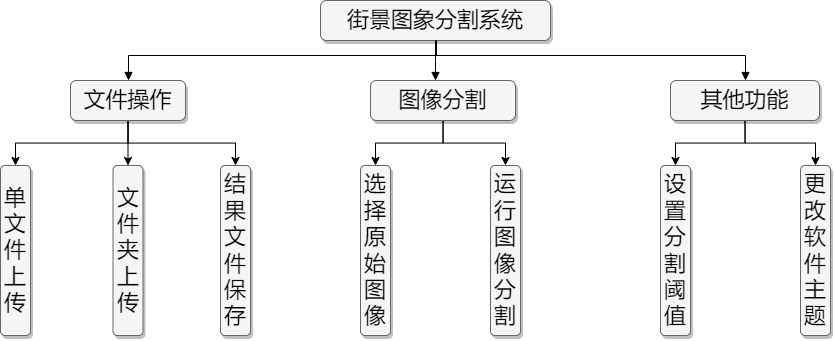
\includegraphics[width=12cm]{fig/chap4/系统架构图1.png}
    \caption{图像分割系统}
    \label{fig:f4a}
\end{figure}

\subsection{系统使用流程}
系统面向专业研究人员使用,为用户制定了具体的业务流程,简要的操作流程如\cref*{fig:f4b}所示。该系统不需要登录注册,仅作为轻量的图像处理工具,即插即用。用户直接进入系统主页面,根据需求上传图片文件或者图片文件夹。上传文件后,可对图像进行一系列基础图像操作,同时支持回退。也可以选择气泡检测功能,检测成功后系统会根据结果输出检测图像和计算的数据共同组成特征数据保存到本地。此上步骤均允许重复操作,每一步的操作结果均会显示在界面上。

\begin{figure}[htb]
    \centering
    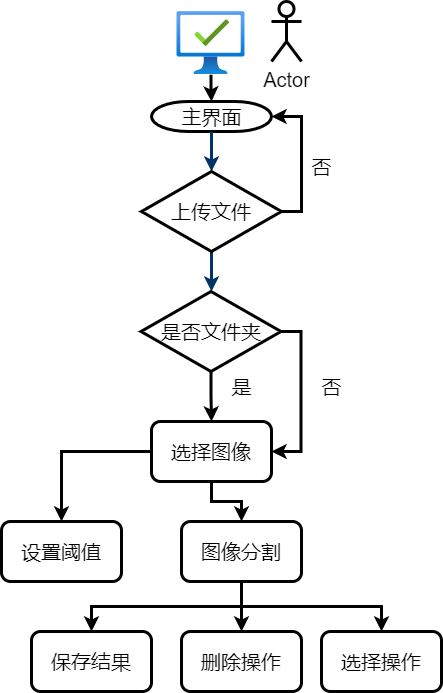
\includegraphics[width=8cm]{fig/chap4/系统流程图2.png}
    \caption{图像分割系统}
    \label{fig:f4b}
\end{figure}

\subsection*{文件操作}
文件操作模块主要涉及到文件上传和结果文件保存模块。文件上传模块提供单文件上传和多文件上传功能。用户选择单文件上传后,系统接收文件并计算图像的基本信息,
然后将这些信息回显到界面中。多文件上传是以文件夹的形式上传多张图像,系统为每张图像设置唯一编号,并在界面中显示编号列表以方便用户查看。
\subsection*{图像分割}
系统提供对所选择图像执行分割处理的操作,同时允许叠加多种图像处理操作,也支持回溯操作,即可以回退到上一步操作,防止用户误操作。用户可以根据最终的分割效果,对分割阈值进行调整,以获得更优的分割效果。
\subsection*{其他功能}
系统提供了软件主题明亮和暗黑的更新功能,软件主题的更换可以满足用户的个性化需求,实现定制化操作界面。 不同的主题可以带来全新的视觉体验,使软件界面显得更加新颖和时尚。主题更换增加了软件的趣味性,可以在一定程度上提高用户的体验度和依赖性。 相比功能更新,主题更换的成本较小,但可以产生较大的新鲜感,这在一定程度上延长了软件的生命周期。
\section{系统运行展示}
\cref*{fig:f4c}为所设计系统暗黑模式下的初始界面,居中部分为图像处理后结果的展示框,界面中下白色框展示图像路径,界面右下为操作按钮。\cref*{fig:f4d}展示了系统的执行过程效果图。
\begin{figure}[htb]
    \centering
    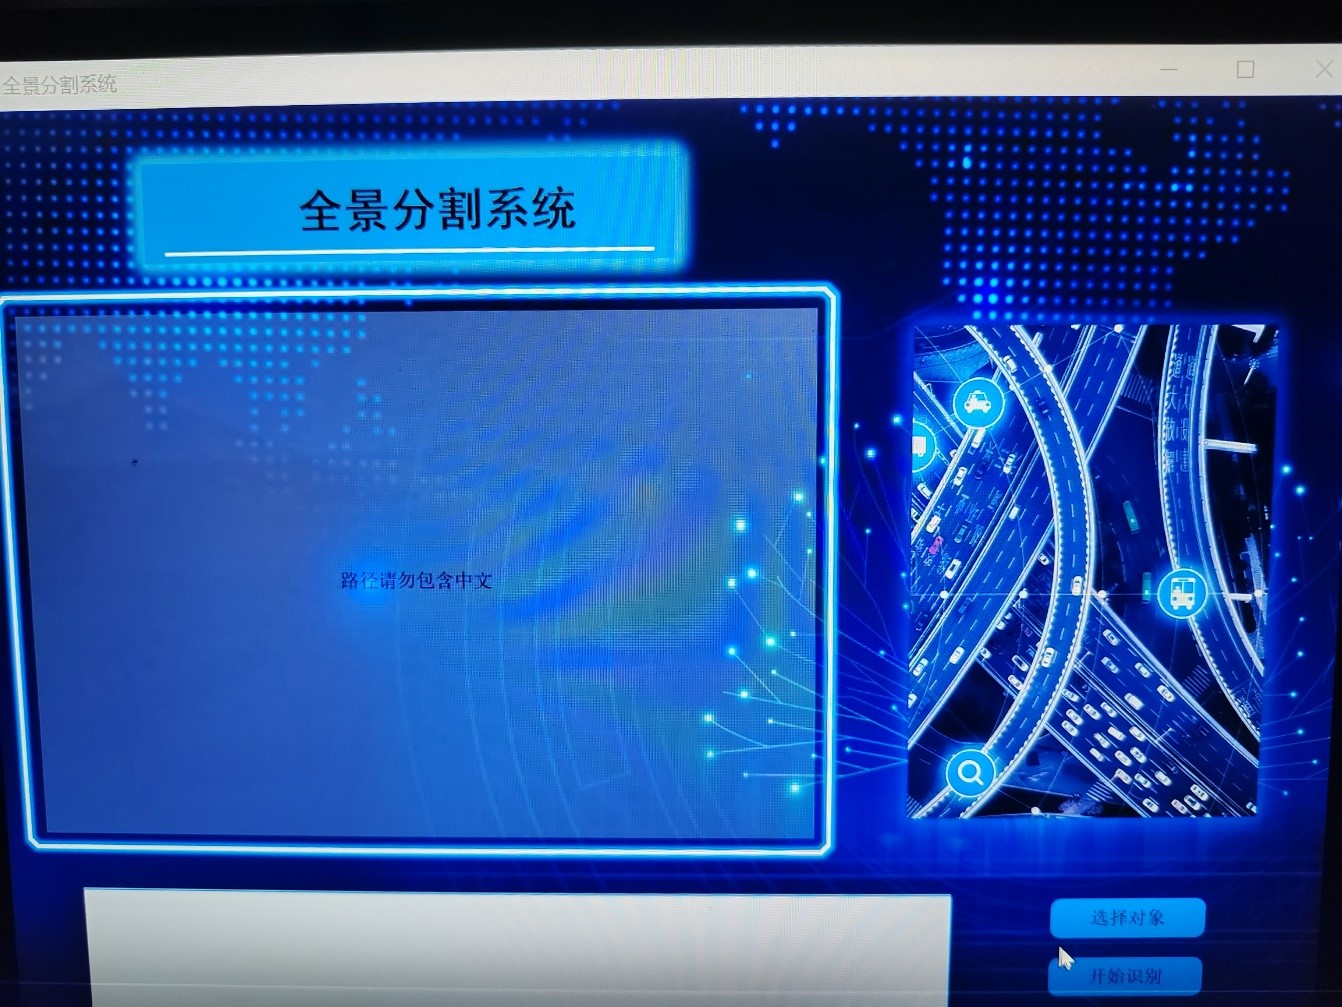
\includegraphics[width=8cm]{fig/chap4/可视化2.jpg}
    \caption{系统初始界面}
    \label{fig:f4c}
\end{figure}


\begin{figure}[htb]
    \centering
    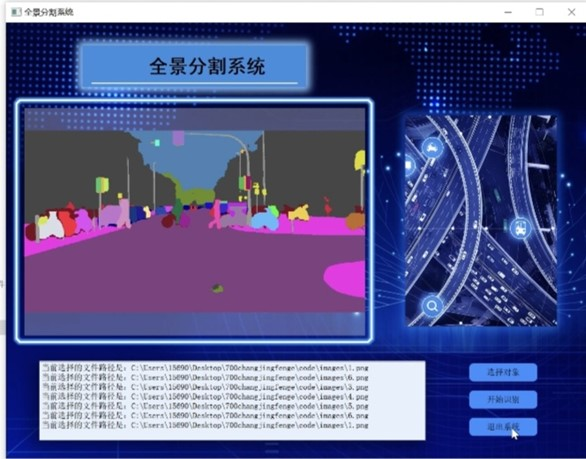
\includegraphics[width=8cm]{fig/chap4/可视化1.jpg}
    \caption{系统分割效果图}
    \label{fig:f4d}
\end{figure}
\subsection*{代码补充说明}
系统前端部分本研究采用PyQt完成软件开发,代码使用QtWidgets、QApplication等模块,编写代码中首先创建QApplication类的一个对象。这一步操作保证了UI应用程序存在入口点。然后使用本文创建QWidget类的一个对象。QWidget是Qt中所有UI对象的基类,本质上在应用程序中看到的所有东西都是一个小部件。包括对话框、文本、按钮、栏等等。官方允许用户设计复杂用户界面的功能,小部件嵌套完成堆叠效果。

系统模型部分,由于pytorch模型依赖于Pytorch框架,本研究为了减少平台依赖度,将PyTorch模型转换为了ONNX模型,ONNX是一个开放的神经网络交换格式,支持PyTorch、TensorFlow、Keras等主流深度学习框架之间的模型转换。转换为ONNX可以使PyTorch模型在更多平台下运行,不再限于PyTorch框架。ONNX模型可以部署到移动端和嵌入式设备。ONNX Runtime使ONNX模型可以高性能地运行在ARM、x86等服务器端和客户端CPU上,以及蓝牙等嵌入式设备上。这使得PyTorch模型得到更广泛的应用场景。ONNX模型具有较小的体积。相比PyTorch模型,ONNX模型提供了更加轻量级的格式,这使其更加适合在资源受限的环境下部署。
\begin{figure}[htb]
    \centering
    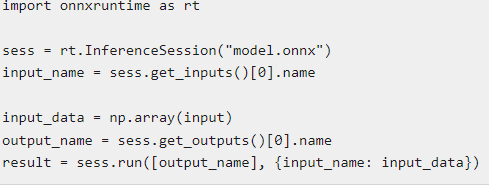
\includegraphics[width=8cm]{fig/chap4/代码图.png}
    \caption{加载ONNX模型实例代码}
    \label{fig:f4e}
\end{figure}

代码第一行,导入ONNX Runtime,用于加载和推理ONNX模型。 第二行,使用InferenceSession类加载ONNX模型。第三行,得到模型输入节点的名称。 第四行,构造模型输入数据。第五行,得到模型输出节点的名称。第六行,使用run方法进行模型推理,输入数据传入输入节点,输出数据从输出节点获得。第七到第十行,输出模型推理结果。



\section{本章小结}
为了更方便研究人员快速、便捷的利用所属的深度学习模型对街景图像的分割处理,帮助后续执行自动驾驶追踪。本章利用 PyQt5 框架,设计开发了一个图像分割系统。系统实现了诸如文件操作、图像分割和其他附加功能,可供专业研究人员快速对街景图像进行处理,同时获取相关图像特征,以便后续利用这些特征与自动驾驶获得的其他特征信息进行建模。

% !TEX root = ../swputhesis.tex
\chapter{总结与展望}
\section{全文总结}
本次研究受到FCOS目标检测器性能的启发,采用设计了一款单阶段全景分割网络,其包括三个分支结构,分别为目标检测、语义和全景分支结构,以此来扩展目标检测器输出的网络特征图。而目标检测器的主要作用在于对实例中心目标进行检测以及感知生成像素级实例掩码。语义分支的主要作用在于给全景分支提供语义标签。计算全景分割结果的原理在于对语义和全景分支网络的像素进行乘积计算。以端对端的学习方式防止网络产生启发式融合冲突问题。本次研究设计的网络架构是自上而下的单阶段结构,推理的难度较小,能够降低深度学习推理的难度,更容易部署实际应用场景。在对比分析数据集的分割可视化效果来看,单阶段架构的分割效果更理想,通过感知像素级实例掩码的方式能够有效提高全景分割的准确性,这样就能够有效的解决全景分割处理二维图像过程中出现的推理准确性和时间不平衡的问题。

\section{工作展望}
为了进一步提高单阶段结构全景分割处理二维图像的准确性,本章节在感知像素级实例掩码的基础上提出了全新的全景分割方法,其主要包括三个分支结构,即目标检测、语义和全景分支结构,以此来增加FCOS目标检测器输出网络特征的结果。而目标检测器的主要作用在于对实例中心目标进行检测以及感知生成像素级实例掩码。语义分支的主要作用在于给全景分支提供语义标签。计算全景分割结果的原理在于对语义和全景分支网络的像素进行乘积计算。本次设计的网络选择的验证和标准数据集是Cityscapes ,那么本次设计的全景分割方法的性能与双阶段全景分割法的性能是非常接近的。在对比验证分割预测和分析可视化程度方面,本次研究在感知像素级实例掩码的基础上提出了全景分割二维图像的方法,能够有效的处理大尺度物体过于分割而小尺度问题分割不足的问题,以此来处理推理时间和进度不平衡的问题,使模型的推理更加容易,便于模型进行深度学习,让布局实际应用场景变得更加容易。

% !TEX root = ../swputhesis.tex
\chapter{附录}
1. 特征提取网络
\begin{lstlisting}	%正文插入代码
    import torch
    import torch.nn as nn
    class PixelwiseFeatureExtractor(nn.Module):
        def __init__(self):
            super(PixelwiseFeatureExtractor, self).__init__()
            # 定义卷积层
            self.conv1 = nn.Conv2d(3, 64, kernel_size=3, stride=1, padding=1)
            self.conv2 = nn.Conv2d(64, 128, kernel_size=3, stride=1, padding=1)
            self.conv3 = nn.Conv2d(128, 256, kernel_size=3, stride=1, padding=1)
            self.conv4 = nn.Conv2d(256, 512, kernel_size=3, stride=1, padding=1)
            self.conv5 = nn.Conv2d(512, 512, kernel_size=3, stride=1, padding=1)
            self.pool = nn.MaxPool2d(kernel_size=2, stride=2)
            self.relu = nn.ReLU(inplace=True)
            self.upsample = nn.Upsample(scale_factor=2, mode='bilinear', align_corners=True)   
        def forward(self, x):
            x1 = self.conv1(x)
            x1 = self.relu(x1)
            x1 = self.pool(x1)
            x2 = self.conv2(x1)
            x2 = self.relu(x2)
            x2 = self.pool(x2)
            x3 = self.conv3(x2)
            x3 = self.relu(x3)
            x3 = self.pool(x3)
            
            x4 = self.conv4(x3)
            x4 = self.relu(x4)
            x4 = self.pool(x4)
            x5 = self.conv5(x4)
            x5 = self.relu(x5)
            x5_up = self.upsample(x5)
            x4_up = self.conv4(x3)
            x4_up = self.relu(x4_up)
            x4_up = torch.cat([x4_up, x5_up], dim=1)
            x4_up = self.upsample(x4_up)
            x3_up = self.conv3(x2)
            x3_up = self.relu(x3_up)
            x3_up = torch.cat([x3_up, x4_up], dim=1)
            x3_up = self.upsample(x3_up)
            x2_up = self.conv2(x1)
            x2_up = self.relu(x2_up)
            x2_up = torch.cat([x2_up, x3_up], dim=1)
            x2_up = self.upsample(x2_up)
            x1_up = self.conv1(x)
            x1_up = self.relu(x1_up)
            x1_up = torch.cat([x1_up, x2_up], dim=1)
            return x1_up
\end{lstlisting}

2.语义分支网络
\begin{lstlisting}	%正文插入代码

    import tensorflow as tf
    def fcn_model(input_shape, num_classes):
        # 定义输入层
        inputs = tf.keras.layers.Input(shape=input_shape)
        # 编码器部分
        conv1 = tf.keras.layers.Conv2D(64, (3, 3), activation='relu', padding='same')(inputs)
        pool1 = tf.keras.layers.MaxPooling2D((2, 2))(conv1)
        conv2 = tf.keras.layers.Conv2D(128, (3, 3), activation='relu', padding='same')(pool1)
        pool2 = tf.keras.layers.MaxPooling2D((2, 2))(conv2)
        conv3 = tf.keras.layers.Conv2D(256, (3, 3), activation='relu', padding='same')(pool2)
        # 解码器部分
        up1 = tf.keras.layers.UpSampling2D((2, 2))(conv3)
        conv4 = tf.keras.layers.Conv2D(128, (3, 3), activation='relu', padding='same')(up1)
        up2 = tf.keras.layers.UpSampling2D((2, 2))(conv4)
        conv5 = tf.keras.layers.Conv2D(64, (3, 3), activation='relu', padding='same')(up2)
        outputs = tf.keras.layers.Conv2D(num_classes, (1, 1), activation='softmax')(conv5)
\end{lstlisting}


3.全景分支网络
\begin{lstlisting}
    import torch
    import torch.nn as nn
    import torch.nn.functional as F
    class PanopticSegNet(nn.Module):
        def __init__(self, num_classes):
            super(PanopticSegNet, self).__init__()
            self.num_classes = num_classes
            
            # Encoder
            self.conv1 = nn.Conv2d(3, 64, kernel_size=3, padding=1)
            self.bn1 = nn.BatchNorm2d(64)
            self.conv2 = nn.Conv2d(64, 128, kernel_size=3, padding=1)
            self.bn2 = nn.BatchNorm2d(128)
            self.conv3 = nn.Conv2d(128, 256, kernel_size=3, padding=1)
            self.bn3 = nn.BatchNorm2d(256)
            self.conv4 = nn.Conv2d(256, 512, kernel_size=3, padding=1)
            self.bn4 = nn.BatchNorm2d(512)
            self.conv5 = nn.Conv2d(512, 1024, kernel_size=3, padding=1)
            self.bn5 = nn.BatchNorm2d(1024)
            # Decoder
            self.upconv1 = nn.ConvTranspose2d(1024, 512, kernel_size=2, stride=2)
            self.bn6 = nn.BatchNorm2d(512)
            self.conv6 = nn.Conv2d(1024, 512, kernel_size=3, padding=1)
            self.bn7 = nn.BatchNorm2d(512)
            self.upconv2 = nn.ConvTranspose2d(512, 256, kernel_size=2, stride=2)
            self.bn8 = nn.BatchNorm2d(256)
            self.conv7 = nn.Conv2d(512, 256, kernel_size=3, padding=1)
            self.bn9 = nn.BatchNorm2d(256)
            self.upconv3 = nn.ConvTranspose2d(256, 128, kernel_size=2, stride=2)
            self.bn10 = nn.BatchNorm2d(128)
            self.conv8 = nn.Conv2d(256, 128, kernel_size=3, padding=1)
            self.bn11 = nn.BatchNorm2d(128)
            self.upconv4 = nn.ConvTranspose2d(128, 64, kernel_size=2, stride=2)
            self.bn12 = nn.BatchNorm2d(64)
            self.conv9 = nn.Conv2d(128, 64, kernel_size=3, padding=1)
            self.bn13 = nn.BatchNorm2d(64)
            # Output
            self.conv10 = nn.Conv2d(64, self.num_classes, kernel_size=1)
        def forward(self, x):
            # Encoder
            x = F.relu(self.bn1(self.conv1(x)))
            x = F.max_pool2d(x, 2)
            x = F.relu(self.bn2(self.conv2(x)))
            x = F.max_pool2d(x, 2)
            x = F.relu(self.bn3(self.conv3(x)))
            x = F.max_pool2d(x, 2)
            x = F.relu(self.bn4(self.conv4(x)))
            x = F.max_pool2d(x, 2)
            x = F.relu(self.bn5(self.conv5(x)))
            # Decoder
            x = F.relu(self.bn6(self.upconv1(x)))
            x = torch.cat([x, self.bn4(self.conv4(x))], dim=1)
            x = F.relu(self.bn7(self.conv6(x)))
            x = F.relu(self.bn8(self.upconv2(x)))
            x = torch.cat([x, self.bn3(self.conv3(x))], dim=1)
            x = F.relu(self.bn9(self.conv7(x)))
            x = F.relu(self.bn10(self.upconv3(x)))
            x = torch.cat([x, self.bn2(self.conv2(x))], dim=1)
            x = F.relu(self.bn11(self.conv8(x)))
            x = F.relu(self.bn12(self.upconv4(x)))
            x = torch.cat([x, self.bn1(self.conv1(x))], dim=1)
            x = F.relu(self.bn13(self.conv9(x)))
            # Output
            x = self.conv10(x)
            x = F.interpolate(x, scale_factor=4, mode='bilinear')
            return x
\end{lstlisting}

4.导入必要的库和模块
\begin{lstlisting}
    import tensorflow as tf
    from tensorflow.keras.applications.resnet50 import ResNet50
    from tensorflow.keras.models import Model
    from tensorflow.keras.layers import Input, Conv2DTranspose, Concatenate, Activation 
\end{lstlisting}

5.定义网络模型
\begin{lstlisting}
    def create_model(input_shape, num_classes):
        # 加载ResNet50-FPN模型
        resnet50_fpn = ResNet50(include_top=False, weights='imagenet', input_shape=input_shape)
        # 获取输出特征图
        C3, C4, C5 = resnet50_fpn.get_layer('conv3_block4_out').output, resnet50_fpn.get_layer('conv4_block6_out').output, resnet50_fpn.output
        # 上采样
        P5 = Conv2DTranspose(filters=256, kernel_size=(3, 3), strides=2, padding='same')(C5)
        P5 = Concatenate()([P5, C4])
        P5 = Conv2DTranspose(filters=256, kernel_size=(3, 3), strides=2, padding='same')(P5)
        P5 = Concatenate()([P5, C3])
        # 分类器
        output = Conv2DTranspose(filters=num_classes, kernel_size=(3, 3), strides=2, padding='same')(P5)
        output = Activation('softmax')(output)
        # 定义模型
        model = Model(inputs=resnet50_fpn.input, outputs=output)
        return model
\end{lstlisting}

6.训练编译模型
\begin{lstlisting}
    model = create_model(input_shape=(256, 256, 3), num_classes=2)
    model.compile(optimizer='adam', loss='categorical_crossentropy', metrics=['accuracy'])
    model.fit(x_train, y_train, batch_size=32, epochs=10, validation_data=(x_val, y_val))
\end{lstlisting}



\backmatter

% 致谢
% !TEX root = ../swputhesis.tex
\chapter{致\hspace{\ccwd}谢}
在攻读硕士学位期间,得到了很多人的指导和鼓励。首先非常由衷地感谢各位同学和老师。

时间过得很快,一眨眼,我的大学生涯就要结束了。在这里,我要向我的家人,老师,以及同学表示感谢,感谢他们对我的帮助和帮助,使我在大学期间过得很充实。
首先,我想对王猛先生表示衷心的感谢。王先生为人谦逊,平易近人,在我的论文中起着至关重要的作用。王先生从第一个题目的选择到后面的文章的撰写,都给了我很好的指导。在我的第一篇文章写完以后,他还在百忙中抽空对我的文章进行了仔细的审阅,并给出了很多有针对性的建议,让我的研究与写作始终没有迷失方向。他严谨的学术态度和对生活的执着精神,将会一直鼓舞和鼓舞我。
其次,我想对河南牧业经济学院所有教师表示衷心的谢意。他们严格,无私,高质量的指导,使我在二年多的时间里,不仅提高了自己的业务水平,而且为我的论文的撰写奠定了良好的理论基础。同时,也要向我的同窗、舍友表示衷心的谢意,感谢你们一直以来对我的支持与支持,使我们的友情更加长久。
当然,我要感谢生养我的父母。他们的关心、支持和鼓励是我成长的重要动力。还有我爱的人,感谢你一路上的支持和鼓励,让我在遇到困难时坚定前行。
最后,我要对评审我的论文的各位指导老师表示诚挚的谢意。感谢你们的认真审阅和指导。我将倍加珍惜这段珍贵的经历和经验,为自己的未来奠定坚实的基础。


% 显示参考文献列表,并加参考文献加入目录
\printbibliography[heading=bibintoc]

% 攻读硕士学位期间发表的论文及科研成果
\include{src/resume}

\end{document}
